\section{Background}\label{sec:background}

Both particle and Kalman filters are types of \emph{recursive Bayesian estimators},
or \emph{Bayes filters} \cite{ref:4}. A Bayes filter provides a probabilistic framework
for estimation, but cannot be instantiated itself \cite{ref:3}. In other words,
particle and Kalman filters are both implementations of the generic Bayes filter.
As such, they share very similar properties, and a designer must go through the
same initial steps for both.\cite{ref:4}

To avoid confusion, the \emph{system} refers to the system whose state we are
attempting to estimate. The Bayes filter uses a \emph{dynamical model} and
\emph{observations} to achieve this. Depending on the context, both
\emph{observations} and \emph{sensor measurements} are used in the text, and
mean the same thing.

\subsection{State Space}\label{sec:state-space}
A Bayes filter is used for estimating the \emph{state} of a dynamic system from
noisy sensor measurements. The dynamic system is described by the state
vector $\textbf{x}$, and the following generic notation is used.

%TODO center this math
\begin{math}
\mathbf{x}_{t}\quad\quad\quad\textrm{state at time t} \\
\mathbf{z}_{t}\quad\quad\quad\textrm{observation at time t} \\
\mathbf{u}_{t}\quad\quad\quad\textrm{system input at time t}
\end{math}

Note that all of the state variables are vectors, indicating that a system can
have multiple states, observations and inputs. To illustrate how a system can be
decomposed into its state space, consider the spring-mass-damper system shown in
Figure \ref{fig:spring-mass-damper}.

\begin{figure}[h]
\centering
\includegraphics[width=0.6\textwidth]{images/cart-system}
\caption{Spring-mass-damper system. $k$ and $C$ are the spring and damping
    coefficients respectively, $p$ is the position referenced from zero and $F$
    the applied force.
}
\label{fig:spring-mass-damper}
\end{figure}

The cart shown in the Figure is anchored
to the wall by a spring and damper. It slides on a frictionless surface and has
unity mass. There is an input $u = F$ which excites the system.

We arbitrarily decide that the state of the system is composed of the two
variables\footnote{Note that we could have chosen any property of the system
as a state variable. Such a simple model offers few options however.}
: position $p$ and velocity $\dot{p}$. We can then use Newton's second law,
$\sum{F} = ma$,
to develop a force balance equation:

\begin{displaymath}
F_{spring} = -kp \\
\end{displaymath}
\begin{displaymath}
F_{damper} = -C\dot{p} \\\\
\end{displaymath}

\begin{align*}
\sum{F} &= ma \\ &= m\ddot{p} \\
&= -C\dot{p} -kp + u
\end{align*}

Which allows us to write a single differential equation to describe the dynamics
of the system.

\begin{equation}
\implies m\ddot{p} + C\dot{p} + kp = u
\end{equation}

The system state consists of position $p$ and velocity $\dot{p}$, and we form
the state vector thus:

\begin{equation}
    \mathbf{x} =
    \begin{bmatrix}
        p \\
        \dot{p}
    \end{bmatrix}
    =
    \begin{bmatrix}
        x_{1} \\
        x_{2}
    \end{bmatrix}
\end{equation}

From which we can create the state space,

\begin{align*}
    \mathbf{\dot{x}}
    &=
    \begin{bmatrix}
        \dot{p} \\
        \ddot{p}
    \end{bmatrix} \\ \\ 
    &=
    \begin{bmatrix}
        \dot{x} \\
        \frac{C}{M}\dot{p} - \frac{k}{M}p
    \end{bmatrix} \\ \\ 
    &=
    \begin{bmatrix}
        x_{1} \\
        \frac{C}{M}x_{2} - \frac{k}{M}x_{1} - u
    \end{bmatrix} \\ \\
    &=
    \begin{bmatrix}
        0 & 1\\
        \frac{-k}{M} & \frac{-C}{M} \\
    \end{bmatrix}
    \begin{bmatrix}
        x_{1} \\
        x_{2}
    \end{bmatrix}
    +
    \begin{bmatrix}
        0 \\
        1
    \end{bmatrix}
    u
\end{align*}

Which has the usual state space form,

\begin{equation}\label{eq:sys-ss}
\mathbf{\dot{x}} = \mathbf{A}\mathbf{x} + \mathbf{B}u
\end{equation}

where

\begin{equation*}
    \mathbf{A} =
    \begin{bmatrix}
        0 & 1\\
        \frac{-k}{M} & \frac{-C}{M} \\
    \end{bmatrix}
    \end{equation*}

    \begin{equation*}
    \mathbf{B} =
    \begin{bmatrix}
        0 \\
        1
    \end{bmatrix}
\end{equation*}

We model the sensors similarly. The values of the matrices depend on which modes
we are able to observe. In this example we have said that we are able to observe
position, but not velocity. Our sensor vector is therefore simply a scalar
value equal to
the first mode (position) of the system:

\begin{equation}
    \mathbf{z} =
    \begin{bmatrix}
        z
    \end{bmatrix}
    = x_{1}
\end{equation}

The state space observation equation is therefore:

\begin{equation}
    z =
    \begin{bmatrix}
        1 & 0
    \end{bmatrix}
    \begin{bmatrix}
        x_{1} \\
        x_{2}
    \end{bmatrix}
    +
    \begin{bmatrix}
        0 \\
        0
    \end{bmatrix}
    u
\end{equation}

which we write using the usual state space notation.

\begin{equation}\label{eq:obs-ss}
z = \mathbf{C}\mathbf{x} + \mathbf{D}u
\end{equation}

These are the key equations used in both the particle and Kalman filtering
algorithms.

Although the derivations of these state space forms are long-winded, the
formation of the state space is an important step for a Bayes filter.

\subsubsection{Discrete System Issues}\label{sec:discrete}
Even though we have the system in state space form, it is not quite ready for
use as a model for a Bayes filter. There is a subtle change in the form of equations
\ref{eq:sys-ss} and \ref{eq:obs-ss} when used to model a discrete system,
such as when modelling using Matlab. The
changes are shown here without justification.\footnote{The reason is to do with
    the fact that a finite time step must be used when implemented digitally.
}

\begin{equation}
\mathbf{x_{t+1}} = \mathbf{F}\mathbf{x_{t}} + \mathbf{G}u_{t}
\end{equation}

\begin{equation}
z_{t} = \mathbf{H}\mathbf{x_{t}} + \mathbf{J}u_{t}
\end{equation}

where
%TODO align these
\begin{equation*}
    \mathbf{F} = \mathrm{\Delta t}\mathbf{A} + \mathbf{I}
    \quad\quad\mathbf{H} = \mathbf{C}
\end{equation*}
\begin{equation*}
\mathbf{G} = \mathrm{\Delta t}\mathbf{B}
\quad\quad\quad\mathbf{J} = \mathbf{D}
\end{equation*}

The reason for these changes is beyond the scope of this discussion and does
not affect any results.

\subsection{Estimation Process}
The aim of the Bayes filter is to find the belief about the current state,

\begin{equation}
Bel(\mathbf{x}_{t}) = p(\mathbf{x}_{t} | \mathbf{z}_{1}, \mathbf{z}_{2}, \dots
, \mathbf{z}_{t})
\end{equation}

that is, the probability of $\mathbf{x}_{t}$ given all the data we've seen so far.
Roughly speaking, the belief answers the question: \emph{What is the probability
that the system's state is $\mathbf{x}$ if the history of sensor measurements is
$\mathbf{z}_{1}, \mathbf{z}_{2}, \dots, \mathbf{z}_{t}$}?

The number of observations grows with time, and will get large very quickly
(withing a few seconds) in any system where measurements are taken at a high rate.
To make the computation tractable,
Bayes filters assume that the dynamic system is a \emph{Markov} process.\cite{ref:4}
The result of this assumption is that we can
assume that the
current state $\mathbf{x}_{t}$ contains all the information we need. Using
the cart example given previously, the Markov assumption implies that sensor measurements
depend only on the carts current position and velocity, and that its position
and velocity (stat) at
time $t$ depends only on the previous state $\mathbf{x}_{t-1}$. That is, states
before $\mathbf{x}_{t-1}$ provide no additional information under this Markov
assumption.

With this assumption made, the belief function simplifies to:

\begin{equation}\label{eq:markov-belief}
Bel(\mathbf{x}_{t}) = p(\mathbf{x}_{t} | \mathbf{z}_{t})
\end{equation}

\subsubsection{Updating the Bayes Filter}\label{sec:updating-bayes}
Whenever a sensor provides a new observation\footnote{
    Although written as a vector generally, it is worth noting that in many systems,
    including the cart system above, there is only a single observation and the
    observation vector has only one element, i.e., it is a scalar}
$\mathbf{z}_{t}$, the filter predicts state according
to (\ref{eq:bayes-predict}). Note that the new sensor observation is not used in this step.

\begin{equation}\label{eq:bayes-predict}
p(\mathbf{x}_{t} | \mathbf{z}_{t-1}) = \int{p(\mathbf{x}_{t} | \mathbf{x}_{t-1})
p(\mathbf{x}_{t} | \mathbf{z}_{t-1})\mathrm{d}\mathbf{x}_{t-1}}
\end{equation}

The filter then corrects the predicted estimate using the new sensor observation
according to\footnote{
We can write (\ref{eq:bayes-update}) as
$\alpha p(\mathbf{z}_{t} | \mathbf{x}_{t})p(\mathbf{x}_{t} | \mathbf{z}_{t-1})$
if we know that the sensor variance does not change with time.
}
    (\ref{eq:bayes-update}).

\begin{equation}\label{eq:bayes-update}
    p(\mathbf{x}_{t} | \mathbf{z}_{t}) =
    \frac
    {p(\mathbf{z}_{t} | \mathbf{x}_{t})p(\mathbf{x}_{t} | \mathbf{z}_{t-1})}
    {p(\mathbf{z}_{t} | \mathbf{z}_{t-1})}\\
\end{equation}

%TODO make a comparison to Bayes Rule

It is often difficult to understand exactly what this all means just by looking at
Equations (\ref{eq:bayes-predict}) and (\ref{eq:bayes-update}).
A more qualitative description is often more helpful for understanding what is
happening.

\begin{compactitem}
\item
$p(\mathbf{z}_{t} | \mathbf{x}_{t})$ is the perceptual model. It is the probability
of seeing a particular observation given that the system is in some state
$\mathbf{x}_{t}$ at time $t$. Using the previous example, it describes the
likelihood of making observation $z$ given that the cart is at location $x$.
The distribution is a property of a given sensor. \\
% TODO if filling required: to plots of good vs bad sensors.
\item
$p(\mathbf{x}_{t} | \mathbf{x}_{t-1})$ is sometimes referred to as the action
model and describes the system dynamics. This is why it is essential to formulate
a state space model of the system under examination, as this is what is used to
formulate the distribution.
\end{compactitem}

At this point it is worth iterating that Bayes filters only provides a
probabilistic framework for recursive state estimation and that implementing
a Bayes filter required specifying the perceptual model
$p(\mathbf{z}_{t} | \mathbf{x}_{t})$, the system dynamics
$p(\mathbf{x}_{t} | \mathbf{x}_{t+1})$ and the representation of the Belief
$p(\mathbf{x}_{t} | \mathbf{z}_{t})$.

\subsection{The Kalman Implementation}
%TODO TODO TODO !!!
The Kalman filter implementation utilises the specified state space system
model described in Section \ref{sec:state-space}. It is assumed that process noise
is added to the state update model thus:

\begin{equation}
\mathbf{x}_{t+1} = \mathbf{Fx}_{t} + \mathbf{Bu}_{t} + \mathbf{w}_t
\end{equation}

Where $\mathbf{w}_t$ is zero mean, normally-distributed noise with convariance
$\mathbf{Q}$, i.e., $\mathbf{w}_{t} \sim N(0, \mathbf{Q})$.

Measurements are made by observing system state thus,

\begin{equation}
\mathbf{z}_{t} = \mathbf{Hx}_{t} + \mathbf{v}_t
\end{equation}

where $\mathbf{v}_{t} \sim N(0, \mathbf{R})$ and $\mathbf{R}$ is the
noise convariance.

\subsubsection{Prediciton}
The next state is predicted blindly according to supplied state model,

\begin{equation}
\mathbf{x}_{t|t-1} = \mathbf{Fx}_{t-1|t-1} + \mathbf{Bu}_{t}
\end{equation}

and the estimate covariance updated according to,

\begin{equation}
\mathbf{P}_{t|t-1} = \mathbf{FP_{t-1|t-1}F^{T}} + \mathbf{Q}
\end{equation}

\subsubsection{Updating}

The steps to update the Kalman filter are as follows,

The \emph{measurement residual} is calculated,
\begin{equation*}
\tilde{\textbf{z}}_t = \textbf{z}_t - \textbf{H}\textbf{x}_{t|t-1}\\
\end{equation*}
and this is used to calculate the \emph{residual covariance},
\begin{equation*}
\textbf{S}_k = \textbf{H} \textbf{P}_{t|t-1} \textbf{H}^\text{T} + \textbf{R}\\
\end{equation*}
which in turn allows calculation of the \emph{optimal Kalman gain},
\begin{equation*}
\textbf{K} = \textbf{P}_{t|t-1}\textbf{H}^\text{T}\textbf{S}_t^{-1}\\
\end{equation*}
Finally, we update the state estimate,
\begin{equation*}
\hat{\textbf{x}}_{t|t} = \hat{\textbf{x}}_{t|t-1} + \textbf{K}\tilde{\textbf{z}}_t\\
\end{equation*}
and the estimate covariance.
\begin{equation*}
\textbf{P}_{t|t} = (\mathbf{I} - \textbf{K} \textbf{H}) \textbf{P}_{t|t-1}
\end{equation*}

The proof of why this works is beyond the scope of this report, and the above
equations are only included to give an idea of what was implemented in Matlab.

\subsection{The Particle Filter Implementation}

% TODO particle filtering algorithm - Check this
A commonly used algorithm used to implement the particle filter is
\emph{sequential importance resampling} (SIR). The SIR algorithm is the 
original particle filter algorithm and approximates the filtering distribution

\begin{equation}
p(x_k|y_0,\ldots,y_k)
\end{equation}

by a weighted set of $P$ particles

\begin{equation}
\{(w^{(L)}_k,x^{(L)}_k)~:~L\in\{1,\ldots,P\}\}.
\end{equation}

The \emph{importance weights} $w^{(L)}_k$ are approximations to the relative
posterior probabilities (or densities) of the particles such that 
$\sum_{L=1}^P w^{(L)}_k = 1$. The values of the \emph{importance weights} is
evaluated to give $w^{(L)}_k$. As in importance sampling, the expectation of a
function $f(\cdot)$ can be approximated as a weighted average

\begin{equation}
\int f(x_k) p(x_k|y_0,\dots,y_k) dx_k \approx \sum_{L=1}^P w^{(L)} f(x_k^{(L)}).
\end{equation}

The integral is not guaranteed to be computationally tractable, and in the 
situations where it is not, the discrete measure may offer an alternative
that is indeed tractable.

% Because the $\int f(x_k) p(x_k|y_0,\dots,y_k) dx_k$ is very hard to find, we use
% the approximation as a replacement. 

\subsubsection{Implementation}
The implementation of the algorithm is rather simple (compared to other particle
filtering algorithms) and it uses composition and rejection.  To generate a
single sample $x$ at $k$ from $p_{x_k|y_{1:k}}(x|y_{1:k})$

\begin{enumerate}
\item Set $p = 1$
\item Uniformly generate $L$ from $\{1,..., P\}$
\item Generate a test $\hat{x}$ from its distribution
  $p_{x_k|x_{k-1}}(x|x_{k-1|k-1}^{(L)})$
\item Generate the probability of $\hat{y}$ using $\hat{x}$ from
  $p_{y|x}(y_k|\hat{x})$ where $y_k$ is the measured value
\item Generate another uniform $u$ from $[0, m_k]$
\item Compare $u$ and $p\left(\hat{y}\right)$
\item
\begin{enumerate}
\item If u is larger then repeat from step 2
\item If u is smaller then save $\hat{x}$ as $x_{k|k}^{(p)}$ and increment p
\end{enumerate}
\item If $p > P$ then quit
\end{enumerate}

The goal is to generate $P$ \emph{particles} at $k$ using only the particles from
$k-1$. This requires that a Markov equation can be written (and computed) to
generate a $x_k$ based only upon $x_{k-1}$. This algorithm uses composition of
the $P$ particles from $k-1$ to generate a particle at $k$ and repeats (steps 2-6)
until $P$ particles are generated at $k$.

This can be more easily visualized if $x$ is viewed as a two-dimensional array.
One dimension is $k$ and the other dimensions is the particle number.  For
example, $x(k,L)$ would be the $L^{th}$ particle at $k$ and can also be written
$x_k^{(L)}$ (as done above in the algorithm).  Step 3 generates a ''potential''
$x_k$ based on a randomly chosen particle ($x_{k-1}^{(L)}$) at time $k-1$ and
rejects or accepts it in step 6.  In other words, the $x_k$ values are generated
using the previously generated $x_{k-1}$.
